\documentclass[greek]{beamer}
\usepackage{amsmath,amsthm} % needed for mathematics
\usepackage{unicode-math}
\usepackage{xltxtra}
\usepackage{graphicx}
\usetheme{CambridgeUS}
\usecolortheme{seagull}
\usepackage{hyperref}
\usepackage{ulem} % underline words package
\usepackage{xgreek}

\usepackage{pgfpages} 
\usepackage{tikz} % package for shapes and more
%\setbeameroption{show notes on second screen}
%\setbeameroption{show only notes}

\setsansfont{Calibri} % it is said that Calibri is the proper font for reading difficulties

\usepackage{multicol} % package for two or more columns

\usepackage{appendixnumberbeamer} % remove page numbering in appendix

\usepackage{polynom} % polynomial divisions package

\usepackage{pgffor} % macros

\setbeamercovered{transparent}
\beamertemplatenavigationsymbolsempty

\newcounter{askisi} % enviroment for exercises
\newenvironment{askisi}[1][]
{
  \refstepcounter{askisi}\par
  \subsection{Άσκηση \theaskisi}
  \begin{frame}[label=Άσκηση\theaskisi,t]{Εξάσκηση \theaskisi}
}{
  \end{frame}
}

\newcounter{lisi} % enviroment for solutions
\newenvironment{lisi}[1][]
{
  \refstepcounter{lisi}\par
  \subsection{Άσκηση \thelisi}
  \begin{frame}[label=Λύση\thelisi,t]{Λύση \thelisi}
}{
  \end{frame}
}

\title{Ευθείες}
\subtitle{Γενική Εξίσωση Ευθείας}
\author[Λόλας]{Κωνσταντίνος Λόλας}
\institute[$10^ο$ ΓΕΛ]{$10^ο$ ΓΕΛ Θεσσαλονίκης}
\date{}

\begin{document}

\begin{frame}
  \titlepage
\end{frame}

\section{Θεωρία}
\begin{frame}{Αχχχχ! Μεγαλώνουμε}
  Μέχρι στιγμής καμαρώνουμε τις ευθείες σε μία μορφή
  $$y=αx+β$$
  \onslide<2-> Αν και όχι πάντα (π.χ. $x=a$)
\end{frame}

\begin{frame}{One equation to rule them all?}
  Τι γνωρίζουμε?
  \begin{enumerate}
    \item<1-> γραμμή ονομάζουμε οποιαδήποτε εξίσωση με τουλάχιστον μία μεταβλητή
    \item<2-> έχουμε δύο περιπτώσεις (λόγω κλίσης $λ$)
    \item<3-> άρα...
  \end{enumerate}
  \onslide<4-> γιατί να μην έχουμε ΜΙΑ εξίσωση και ας μην έχουμε $λ$.
  \centering
  \only<4->{
    
\includegraphics[width=0.4\textwidth]{"../images/duh.jpeg"}}

\end{frame}

\begin{frame}{YEAHHHHH!}
  Θα μας έκανε κάτι τέτοιο?
  $$Αx+Βy+Γ=0 \text{, με } Α^2+Β^2\ne 0$$
  \centering
  
\includegraphics[width=0.4\textwidth]{"../images/feelsgood.png"}
\end{frame}

\begin{frame}{Check 1!}
  Υπάρχει η $y=αx+β$ στην $Αx+Βy+Γ=0 \text{, με } Α^2+Β^2\ne 0$?

  \onslide<2-> Φυσικά, αρκεί $Β\ne 0$
  \begin{align*}
    Αx+Βy+Γ=0 \\
    Βy=-Αx-Γ  \\
    y=-\frac{Α}{Β}x-\frac{Γ}{Β}
  \end{align*}
  \only<2>{
    \centering
    
\includegraphics[width=0.2\textwidth]{"../images/h1.png"}}
\end{frame}

\begin{frame}{Check 2!}
  Υπάρχει η $x=α$ στην $Αx+Βy+Γ=0 \text{, με } Α^2+Β^2\ne 0$?

  \onslide<2-> Φυσικά, αρκεί $Β=0$ και $Α\ne 0$
  \begin{align*}
    Αx+0y+Γ=0 \\
    Αx=-Γ     \\
    x=-\frac{Γ}{Α}
  \end{align*}
  \only<2>{
    \centering
    
\includegraphics[width=0.2\textwidth]{"../images/h1.png"} 
\includegraphics[width=0.2\textwidth]{"../images/h2.png"}}
\end{frame}

\begin{frame}{\scalebox{-1}[1]{Check 1!}}
  Γράφεται η $y=αx+β$ στην $Αx+Βy+Γ=0 \text{, με } Α^2+Β^2\ne 0$?

  \onslide<2-> Φυσικά
  \begin{align*}
    y=αx+β \\
    αx-1y+β=0
  \end{align*}
  \only<2>{
    \centering
    
\includegraphics[width=0.2\textwidth]{"../images/h1.png"} 
\includegraphics[width=0.2\textwidth]{"../images/h2.png"} 
\includegraphics[width=0.2\textwidth]{"../images/h3.png"}}
\end{frame}

\begin{frame}{\scalebox{-1}[1]{Check 2!}}
  Γράφεται η $x=α$ στην $Αx+Βy+Γ=0 \text{, με } Α^2+Β^2\ne 0$?

  \onslide<2-> Φυσικά
  \begin{align*}
    x=α \\
    1x+0y-α=0
  \end{align*}
  \only<2>{
    \centering
    
\includegraphics[width=0.2\textwidth]{"../images/h1.png"} 
\includegraphics[width=0.2\textwidth]{"../images/h2.png"} 
\includegraphics[width=0.2\textwidth]{"../images/h3.png"} 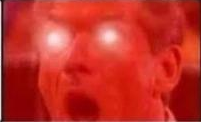
\includegraphics[width=0.2\textwidth]{"../images/h4.png"}}
\end{frame}

\begin{frame}{Μα γιατί να ασχοληθούμε???}
  Μπορούμε να βρίσκουμε άμεσα το παράλληλο στην ευθεία διάνυσμα
  \begin{block}{Το παράλληλο 1}
    Αν $Β\ne 0$ γράφεται ως εξής $y=-\dfrac{Α}{Β}x-\dfrac{Γ}{Β}$, άρα ένα διάνυσμα παράλληλό της είναι το $$(-Β,Α)$$
  \end{block}
  \begin{block}{Το παράλληλο 2}
    Αν $Β= 0$ και $Α\ne 0$ τότε ένα παράλληλο είναι το $(0,Α)$ (γιατί?) άρα και πάλι το $$(-Β,Α)$$
  \end{block}
\end{frame}

\begin{frame}{Γιατί όχι και κάθετα?}
  Αφού η ευθεία είναι παράλληλη στο $(-Β,Α)$
  \begin{block}{Το κάθετο}
    η ευθεία $Αx+Βy+Γ=0$ είναι κάθετη στο διάνυσμα $(Α,Β)$
  \end{block}

\end{frame}

\begin{frame}{Από εδώ και πέρα?}
  Παρατηρήσεις:
  \begin{enumerate}
    \item<1-> ξανά τις ασκήσεις από άλλη σκοπιά
    \item<2-> θα ξέρουμε κατ' ευθείαν την παράλληλη σε διάνυσμα ευθεία
    \item<3-> θα ξέρουμε κατ' ευθείαν την κάθετη σε διάνυσμα ευθεία
    \item<4-> θα ξέρουμε κατ' ευθείαν τις συμμετρικές ως προς άξονες ευθείες
  \end{enumerate}
\end{frame}

\begin{frame}[noframenumbering]
  Στο moodle θα βρείτε τις ασκήσεις που πρέπει να κάνετε, όπως και αυτή τη παρουσίαση
\end{frame}

\section{Ασκήσεις}

\begin{frame}[noframenumbering]
  \vfill
  \centering
  \begin{beamercolorbox}[sep=8pt,center,shadow=true,rounded=true]{title}
    \usebeamerfont{title}Ασκήσεις
  \end{beamercolorbox}
  \vfill
\end{frame}

\begin{askisi} Δίνεται η ευθεία $ε:2x+3y-6=0$. Να βρείτε:
  \begin{enumerate}
    \item<1-> την ευθεία $ζ$ που είναι παράλληλη στην ευθεία $ε$ και διέρχεται από το σημείο $Α(-1,2)$
    \item<2-> τα σημεία τομής της ευθείας $ζ$ με τους άξονες
  \end{enumerate}

  % \hyperlink{Λύση1}{\beamerbutton{Λύση}}
\end{askisi}

\begin{askisi} Να αποδείξετε ότι οι ευθείες
  $$ε_1:x-3y+2=0 \qquad ε_2:2x-y-1=0 \qquad ε_3:5x-3y-2=0$$
  διέρχονται από το ίδιο σημείο

  %\hyperlink{Λύση2}{\beamerbutton{Λύση}}
\end{askisi}

\begin{askisi} Δίνεται η εξίσωση:
  $$(λ^2-1)x+(λ^2-λ)y+λ+1=0,λ\in\mathbb{R}$$
  Να βρείτε για ποιες τιμές του $λ$ η εξίσωση παριστάνει:
  \begin{enumerate}
    \item<1-> ευθεία
    \item<2-> ευθεία παράλληλη στον άξονα $x'x$
    \item<3-> ευθεία παράλληλη στον άξονα $y'y$
  \end{enumerate}

  %\hyperlink{Λύση3}{\beamerbutton{Λύση}}
\end{askisi}

\begin{askisi} Δίνονται οι ευθείες:
  \begin{itemize}
    \item $ε_1:(μ-1)x-(μ-2)y-μ=0$
    \item $ε_2:(μ-2)x-(μ+1)y-3=0$
  \end{itemize}
  Να βρείτε το $μ$ ώστε:
  \begin{enumerate}
    \item<1-> οι ευθείες $ε_1$ και $ε_2$ να τέμνονται
    \item<2-> $ε_1 \parallel ε_2$
    \item<3-> $ε_1 \perp ε_2$
  \end{enumerate}

  %\hyperlink{Λύση4}{\beamerbutton{Λύση}}
\end{askisi}

\begin{askisi} Να βρείτε την οξεία γωνία των ευθειών
  $$ε_1:y=(-2+\sqrt{3})x$$
  και
  $$ε_2:y=-x$$
  %\hyperlink{Λύση5}{\beamerbutton{Λύση}}
\end{askisi}

\begin{askisi} Να βρείτε τις ευθείες που διέρχονται από το σημείο $Ρ(1,-1)$ και σχηματίζουν με την ευθεία $η:x+y-1=0$ οξεία γωνία ίση με $45^{\circ}$

  %\hyperlink{Λύση6}{\beamerbutton{Λύση}}
\end{askisi}

\begin{askisi} Να αποδείξετε ότι όλες οι ευθείες που ορίζονται από την εξίσωση:
  $$ε_λ:(λ+1)x+(λ-1)y+2λ=0 \text{, όπου } λ\in\mathbb{R}$$
  διέρχονται από το ίδιο σημείο $Α$ και στη συνέχεια, να βρείτε εκείνη την ευθεία $ε$ που ορίζεται από την εξίσωση αυτή και είναι κάθετη στην ευθεία $ζ:y=2x$
  %\hyperlink{Λύση}{\beamerbutton{Λύση}}
\end{askisi}

\begin{askisi} Δίνεται η εξίσωση: $x^2-3y^2-2x+1=0$
  \begin{enumerate}
    \item<1-> Να αποδείξετε ότι παριστάνει δύο ευθείες $ε_1$ και $ε_2$ συμμετρικές ως προς τον άξονα $x'x$
    \item<2-> Να βρείτε την οξεία γωνία που σχηματίζουν οι ευθείες $ε_1$ και $ε_2$
  \end{enumerate}

  %\hyperlink{Λύση8}{\beamerbutton{Λύση}}
\end{askisi}

% \appendix
% \section{Λύσεις Ασκήσεων}
% \begin{frame}
%  \tableofcontents
% \end{frame}
% 
% regex
% (\\subsection\{Άσκηση)().*\n.*
% \begin{askisi}
%   \end{frame}
% \end{askisi}

\end{document}
